\documentclass[14pt,a4paper]{extarticle}
\usepackage[T2A]{fontenc}
\usepackage[utf8]{inputenc}
\usepackage[russian]{babel}
\usepackage[left=3cm,right=1.5cm,top=2cm,bottom=2cm]{geometry}
\usepackage{amsmath,amssymb}
\usepackage{graphicx}
\usepackage{booktabs}
\usepackage{array}
\sloppy
\usepackage{setspace}
\usepackage{indentfirst}
\usepackage{caption}
\usepackage{listings}
\usepackage[colorlinks=false,pdfborder={0 0 1},linkbordercolor={1 0 0},citebordercolor={0 1 0},urlbordercolor={0 1 1}]{hyperref}

\setstretch{1.15}
\setlength{\parindent}{1.25cm}
\captionsetup{labelsep=colon,font=small}
\captionsetup[table]{name=Таблица,position=below}
\captionsetup[figure]{name=Рис.,position=below}
\renewcommand{\lstlistingname}{Листинг}
\captionsetup[lstlisting]{position=below,labelsep=colon}

\lstset{
  language=Python,
  basicstyle=\ttfamily\footnotesize,
  keywordstyle=\bfseries,
  columns=fullflexible,
  keepspaces=true,
  frame=single,
  breaklines=true,
  aboveskip=6pt,
  belowskip=6pt
}

\newcommand{\sd}{\ensuremath{\pm}}

\begin{document}

% ---------------- Титульный лист ----------------
\begin{titlepage}
\thispagestyle{empty}
\centering
МИНИСТЕРСТВО НАУКИ И ВЫСШЕГО ОБРАЗОВАНИЯ\\
РОССИЙСКОЙ ФЕДЕРАЦИИ\\[2pt]
ФЕДЕРАЛЬНОЕ ГОСУДАРСТВЕННОЕ БЮДЖЕТНОЕ\\
ОБРАЗОВАТЕЛЬНОЕ УЧРЕЖДЕНИЕ ВЫСШЕГО ОБРАЗОВАНИЯ\\
«ВЯТСКИЙ ГОСУДАРСТВЕННЫЙ УНИВЕРСИТЕТ»\\[2pt]
Институт математики и информационных систем\\
Факультет автоматики и вычислительной техники\\
Кафедра электронных вычислительных машин\\[3.5cm]
{\Large Отчёт по лабораторной работе №3}\\[4pt]
по дисциплине\\[4pt]
«Основы машинного обучения»\\[4pt]
«Метрические методы и метод опорных векторов»\\[3.5cm]
\begin{flushleft}
Выполнил студент гр. ИВТб-2303-06-00 \hfill /Перевозчиков Д.А./\\[1.2cm]
Проверил \hfill /Пащенко Д. Э./
\end{flushleft}
\vfill
Киров\\
2026
\end{titlepage}

% ---------------- 1 ----------------
\section{Цель работы}

Освоить построение метрических и максимизирующих зазор моделей, научиться корректно подбирать их гиперпараметры и сравнить kNN и SVM в воспроизводимом вычислительном эксперименте. В работе вручную реализуется kNN-классификатор в NumPy с проверкой по \texttt{KNeighborsClassifier}; затем на наборе mfeat-karhunen исследуются влияние масштаба признаков, подбор параметров kNN, линейный и RBF-SVM, вычислительная стоимость моделей и решающие области, после чего выбранная модель однократно оценивается на тестовой выборке.

% ---------------- 2 ----------------
\section{Вариант и данные}

Вариант 4: набор mfeat-karhunen (OpenML, data\_id = 16), файл \texttt{variant\_04.csv}, целевой столбец \texttt{class}. Набор содержит 2000 объектов и 64 исходных признака \texttt{att1}--\texttt{att64}.

\emph{Особенности набора:} все 64 признака являются числовыми (коэффициенты Кархунена--Лоэва, описывающие форму объектов). Пропуски отсутствуют, столбцов-идентификаторов нет. Полных дубликатов 6, они оставлены. Классов 10, каждый содержит ровно 200 объектов (рисунок~\ref{fig:classes}), поэтому методы борьбы с дисбалансом не требуются, а macro-усреднение метрик применяется для равного учёта классов.

\begin{table}[h!]
\centering
\begin{tabular}{p{4.6cm}p{9.4cm}}
\toprule
Параметр & Значение \\
\midrule
Версии библиотек & NumPy 2.5.3, pandas 3.0.6, scikit-learn 1.9.1 \\
SEED & 42 \\
Разбиение & Train / Validation / Test = 60 / 20 / 20, стратифицированное: 1200 / 400 / 400 объектов \\
Кросс-валидация & StratifiedKFold(n\_splits=5, shuffle=True, random\_state=42) на Train; одни и те же фолды для всех семейств \\
Метрики & macro-F1 (основная), Accuracy, balanced accuracy; confusion matrix, classification report \\
Preprocessing & числовые признаки: импутация медианой и StandardScaler; включён в Pipeline и обучается заново в каждом фолде; категориальных признаков нет \\
Правило выбора & семейство с наибольшим validation macro-F1; затем переобучение на Train+Validation (1600 объектов) и однократная оценка на Test \\
\bottomrule
\end{tabular}
\caption{Параметры экспериментального протокола}
\label{tab:protocol}
\end{table}

\begin{figure}[h!]
\centering
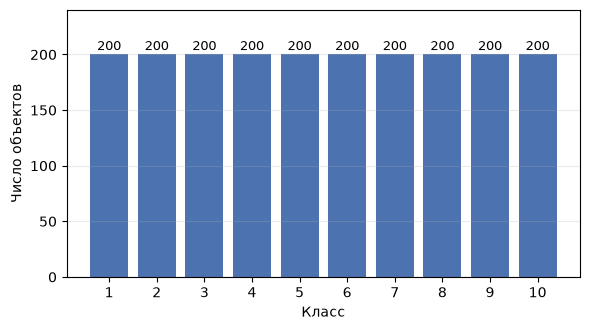
\includegraphics[width=0.62\textwidth]{images/class_dist.png}
\caption{Распределение объектов по классам}
\label{fig:classes}
\end{figure}

На рисунке~\ref{fig:features} показаны два графика признаков: распределение \texttt{att1} по классам и расположение объектов в плоскости (att1, att2). Признак \texttt{att1} хорошо разделяет классы 1, 7 и 8, тогда как классы 4 и 6 имеют широкий разброс, а в плоскости (att1, att2) классы 2, 3, 4 и 9 заметно перемешаны. Ожидаемые сложности: перекрытие классов в пространстве отдельных признаков и высокая размерность (64 признака), при которой расстояния становятся менее различимыми.

\begin{figure}[h!]
\centering
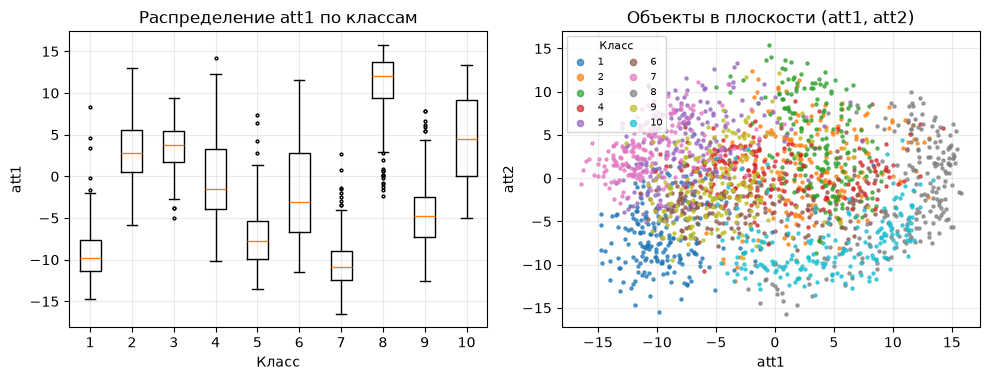
\includegraphics[width=\textwidth]{images/features.png}
\caption{Признак att1 по классам и объекты в плоскости (att1, att2)}
\label{fig:features}
\end{figure}

% ---------------- 3 ----------------
\section{Краткие теоретические сведения}

\textbf{Гипотеза компактности} утверждает, что близкие объекты, как правило, относятся к одному классу. Это не универсальный закон: применимость гипотезы зависит от признакового описания и метрики.

\textbf{Расстояние Минковского.} Расстояние между объектами $x$ и $z$ задаётся формулой
\[
\rho(x,z)=\Bigl(\sum_j |x_j-z_j|^p\Bigr)^{1/p},\quad p\ge 1,
\]
при $p=1$ получается манхэттенское расстояние, при $p=2$ --- евклидово. Если один признак измеряется единицами, а другой тысячами, второй почти полностью определяет расстояние, поэтому признаки стандартизуют: $z_j=(x_j-\mu_{j,\mathrm{train}})/\sigma_{j,\mathrm{train}}$, где $\mu$ и $\sigma$ вычисляются только по Train и переоцениваются заново в каждом фолде кросс-валидации.

\textbf{Метод k ближайших соседей.} Для нового объекта обучающие объекты упорядочиваются по расстоянию, класс определяется голосованием первых $k$ соседей:
\[
\Gamma_c(x)=\sum_{i=1}^{k}[y^{(i)}=c]\,w_i(x),
\]
при равных весах $w_i=1$, при взвешивании по расстоянию $w_i=1/(\rho(x,x^{(i)})+\varepsilon)$. Малое $k$ создаёт сложную границу и повышает дисперсию, большое $k$ сглаживает границу и может привести к недообучению. kNN --- ленивое обучение: этап fit в основном сохраняет Train, основные затраты приходятся на predict.

\textbf{Линейный SVM и максимальный зазор.} Линейный SVM ищет гиперплоскость с максимальной шириной полосы между классами; для неразделимой выборки минимизируется
\[
Q(w)=\tfrac12\|w\|^2+C\sum_i \max\bigl(0,\,1-y_i(\langle w,x_i\rangle-w_0)\bigr).
\]
Первое слагаемое расширяет зазор, второе штрафует за объекты внутри полосы и ошибки. Объекты на границе полосы и нарушающие зазор называются опорными векторами; их число и доля от Train характеризуют сложность модели. Класс \texttt{SVC} реализует многоклассовое решение по схеме one-versus-one.

\textbf{RBF-ядро.} Замена скалярного произведения $\langle x,z\rangle$ ядром $K(x,z)=\exp(-\gamma\|x-z\|^2)$ позволяет строить нелинейную границу без явного вычисления нового признакового пространства. Параметр $\gamma$ задаёт радиус влияния отдельного объекта: малое $\gamma$ --- гладкая граница, большое --- узкие области вокруг отдельных объектов.

\textbf{Основные параметры моделей} приведены в таблице~\ref{tab:params}.

\begin{table}[h!]
\centering
\begin{tabular}{p{3.6cm}p{5.2cm}p{5.2cm}}
\toprule
Параметр & Малое значение & Большое значение \\
\midrule
$k$ & сложная граница, высокая дисперсия & сильное сглаживание, смещение \\
$p$ & ромбовидные окрестности ($p=1$) & круговые окрестности ($p=2$) \\
Вес расстояния & близкие и дальние равноправны & ближайшие доминируют \\
$C$ & больше нарушений ради более широкого зазора & сильнее штраф за нарушения, чувствительность к шуму \\
$\gamma$ (RBF) & широкое влияние, гладкая граница & узкие области вокруг объектов \\
\bottomrule
\end{tabular}
\caption{Основные параметры kNN и SVM}
\label{tab:params}
\end{table}

% ---------------- 4 ----------------
\section{Ход работы и результаты}

\subsection{Константный baseline}

\texttt{DummyClassifier(strategy="most\_frequent")} обучен на Train (1200 объектов) и оценён на Validation (400 объектов): Accuracy = 0.1000, balanced accuracy = 0.1000, macro-F1 = 0.0182. Это нижняя граница качества, которую должны превосходить все последующие модели.

\subsection{Ручная реализация kNN}

kNN реализован средствами NumPy: для каждого объекта вычисляются евклидовы расстояния до всех объектов Train, соседи выбираются сортировкой (\texttt{mergesort}), голоса суммируются по классам с равными весами или с весами $1/\rho$; при совпадении объекта с одним из соседей голосуют только соседи с нулевым расстоянием, при равенстве голосов выбирается минимальная метка (листинг~\ref{lst:knn}).

\begin{lstlisting}[caption={Ядро ручной реализации kNN},label={lst:knn}]
distances = np.sqrt(np.sum((X_train - query) ** 2, axis=1))
order = np.argsort(distances, kind="mergesort")[:k]
neighbor_labels = y_train[order]
neighbor_distances = distances[order]

if weighted and np.any(neighbor_distances <= 1e-12):
    weights = (neighbor_distances <= 1e-12).astype(float)
elif weighted:
    weights = 1.0 / neighbor_distances
else:
    weights = np.ones(k, dtype=float)

scores = {}
for label, weight in zip(neighbor_labels, weights):
    scores[label] = scores.get(label, 0.0) + float(weight)
predictions.append(max(sorted(scores), key=scores.get))
\end{lstlisting}

Проверка выполнена на первых 50 объектах Validation при $k=5$, весах по расстоянию и $p=2$; Train, preprocessing и параметры одинаковы у ручной и библиотечной моделей. Доля совпадений прогнозов равна 1.0 (50 из 50), расхождений нет.

\subsection{Влияние масштабирования признаков}

Для эксперимента второй признак (\texttt{att2}) умножен на 100 на Train и Validation; сравнивались два kNN ($k=11$, веса по расстоянию): с StandardScaler и без него (импутация сохранена). Обе модели обучены на одном и том же Train с искажённым признаком. Для сравнения соседей использованы первые 50 объектов Validation; эталоном служит kNN со стандартизацией на исходных данных (таблица~\ref{tab:scaling}).

\begin{table}[h!]
\centering
\begin{tabular}{llcc}
\toprule
Данные & Scaling & macro-F1 & Доля общих соседей \\
\midrule
исходные  & да  & 0.9403 & 1.0000 \\
исходные  & нет & 0.9750 & 0.7345 \\
att2 $\times$ 100 & да  & 0.9403 & 1.0000 \\
att2 $\times$ 100 & нет & 0.5515 & 0.0818 \\
\bottomrule
\end{tabular}
\caption{Ближайшие соседи и validation macro-F1 до и после искажения масштаба}
\label{tab:scaling}
\end{table}

Со стандартизацией результат не изменился при искажении масштаба: macro-F1 = 0.9403 и множество соседей совпадает с эталоном (доля общих соседей 1.0000). Без стандартизации искажённый признак доминирует в расстоянии: macro-F1 падает до 0.5515, общими с эталоном остаются лишь 8.18\% соседей. На исходных данных без стандартизации macro-F1 равен 0.9750, доля общих соседей --- 0.7345.

\subsection{Подбор параметров kNN}

Подбор выполнен \texttt{GridSearchCV} (scoring = \texttt{f1\_macro}) по сетке $k\in\{1,3,5,7,11,15,21,31\}$, weights $\in$ \{uniform, distance\}, $p\in\{1,2\}$ (32 конфигурации) на стратифицированной 5-кратной CV по Train; preprocessing входит в Pipeline (листинг~\ref{lst:grid}).

\begin{lstlisting}[caption={Подбор параметров kNN в Pipeline},label={lst:grid}]
knn_variant_pipeline = Pipeline([
    ("preprocess", clone(preprocessor)),
    ("model", KNeighborsClassifier()),
])
knn_variant_grid = {
    "model__n_neighbors": [1, 3, 5, 7, 11, 15, 21, 31],
    "model__weights": ["uniform", "distance"],
    "model__p": [1, 2],
}
knn_search_v = GridSearchCV(
    knn_variant_pipeline, knn_variant_grid,
    scoring="f1_macro", cv=variant_cv,
    n_jobs=-1, refit=True, return_train_score=True,
)
knn_search_v.fit(X_train_v, y_train_v)
\end{lstlisting}

Лучшая конфигурация: $k=3$, weights = distance, $p=1$; CV macro-F1 = $0.9407\sd 0.0120$. На Validation она даёт Accuracy = 0.9625, balanced accuracy = 0.9625, macro-F1 = 0.9628. Десять лучших конфигураций приведены в таблице~\ref{tab:knn}, зависимость качества от $k$ --- на рисунке~\ref{fig:knncv}.

\begin{table}[h!]
\centering
\begin{tabular}{cccc}
\toprule
$k$ & weights & $p$ & CV macro-F1 ($\text{среднее}\sd\text{std}$) \\
\midrule
3  & distance & 1 & $0.9407\sd 0.0120$ \\
5  & distance & 2 & $0.9398\sd 0.0193$ \\
1  & distance & 1 & $0.9388\sd 0.0221$ \\
1  & uniform  & 1 & $0.9388\sd 0.0221$ \\
5  & distance & 1 & $0.9381\sd 0.0195$ \\
3  & uniform  & 1 & $0.9368\sd 0.0173$ \\
3  & distance & 2 & $0.9340\sd 0.0092$ \\
7  & distance & 2 & $0.9339\sd 0.0191$ \\
15 & distance & 1 & $0.9313\sd 0.0193$ \\
11 & distance & 1 & $0.9312\sd 0.0217$ \\
\bottomrule
\end{tabular}
\caption{Десять лучших конфигураций kNN по CV macro-F1}
\label{tab:knn}
\end{table}

\begin{figure}[h!]
\centering
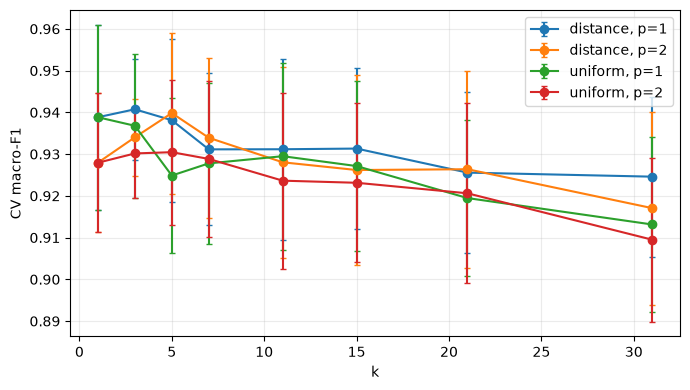
\includegraphics[width=0.85\textwidth]{images/knn_cv.png}
\caption{CV macro-F1 kNN в зависимости от $k$, weights и $p$ (планки --- стандартное отклонение по фолдам)}
\label{fig:knncv}
\end{figure}

Качество максимально при малых $k$ (1--5) и убывает с ростом $k$: при $k=31$ CV macro-F1 равен 0.9246 (distance, $p=1$) и 0.9095 (uniform, $p=2$). При $k=1$ веса не влияют на результат (0.9388 при $p=1$ и 0.9279 при $p=2$), так как есть один сосед. Разница между пятью лучшими конфигурациями (0.9381--0.9407) меньше стандартного отклонения по фолдам (0.012--0.022), поэтому они статистически не различимы.

\subsection{Линейный и RBF-SVM}

Отношение численности самого частого класса к самому редкому в Train равно 1, поэтому \texttt{class\_weight="balanced"} не проверялся. Для линейного SVM проверены $C\in\{0.01;0.1;1;10;100\}$, для RBF-SVM совместно $C\in\{0.1;1;10;100\}$ и $\gamma\in\{\text{scale};0.01;0.1;1\}$ (та же CV, листинг~\ref{lst:svm}).

\begin{lstlisting}[caption={Подбор линейного и RBF-SVM},label={lst:svm}]
linear_variant_pipeline = Pipeline([
    ("preprocess", clone(preprocessor)),
    ("model", SVC(kernel="linear")),
])
linear_search_v = GridSearchCV(
    linear_variant_pipeline,
    {"model__C": [0.01, 0.1, 1.0, 10.0, 100.0],
     "model__class_weight": weight_options},
    scoring="f1_macro", cv=variant_cv, n_jobs=-1, refit=True,
)
rbf_variant_pipeline = Pipeline([
    ("preprocess", clone(preprocessor)),
    ("model", SVC(kernel="rbf")),
])
rbf_search_v = GridSearchCV(
    rbf_variant_pipeline,
    {"model__C": [0.1, 1.0, 10.0, 100.0],
     "model__gamma": ["scale", 0.01, 0.1, 1.0],
     "model__class_weight": weight_options},
    scoring="f1_macro", cv=variant_cv, n_jobs=-1, refit=True,
)
\end{lstlisting}

Результаты сведены в таблице~\ref{tab:svm}. Лучший линейный SVM: $C=0.01$; лучший RBF-SVM: $C=10$, $\gamma=0.01$.

\begin{table}[h!]
\centering
\footnotesize\setlength{\tabcolsep}{3pt}
\begin{tabular}{lcccccc}
\toprule
Модель & CV macro-F1 & Acc & bal.\,acc & macro-F1 & Опорных векторов & Доля \\
\midrule
kNN & $0.9407\sd 0.0120$ & 0.9625 & 0.9625 & 0.9628 & --- & --- \\
Linear SVM & $0.9549\sd 0.0097$ & 0.9625 & 0.9625 & 0.9625 & 696 & 0.5800 \\
RBF SVM & $0.9700\sd 0.0119$ & 0.9775 & 0.9775 & 0.9775 & 790 & 0.6583 \\
\bottomrule
\end{tabular}
\caption{Лучшие конфигурации семейств: CV и validation-метрики (Acc, bal.\,acc, macro-F1 --- на Validation; Доля --- доля опорных векторов от Train)}
\label{tab:svm}
\end{table}

Влияние $C$ для линейного SVM показано в таблице~\ref{tab:lin}, совместное влияние $C$ и $\gamma$ для RBF-SVM --- в таблице~\ref{tab:rbf}.

\begin{table}[h!]
\centering
\begin{tabular}{ccc}
\toprule
$C$ & CV macro-F1 (среднее) & std \\
\midrule
0.01 & 0.9549 & 0.0097 \\
0.1  & 0.9365 & 0.0125 \\
1    & 0.9298 & 0.0096 \\
10   & 0.9298 & 0.0096 \\
100  & 0.9298 & 0.0096 \\
\bottomrule
\end{tabular}
\caption{Влияние $C$ на CV macro-F1 линейного SVM}
\label{tab:lin}
\end{table}

\begin{table}[h!]
\centering
\begin{tabular}{crrrr}
\toprule
$C \backslash \gamma$ & 0.01 & 0.1 & 1.0 & scale \\
\midrule
0.1  & 0.9199 & 0.3315 & 0.0518 & 0.9234 \\
1    & 0.9658 & 0.8032 & 0.0887 & 0.9683 \\
10   & 0.9700 & 0.8153 & 0.1028 & 0.9674 \\
100  & 0.9700 & 0.8153 & 0.1028 & 0.9674 \\
\bottomrule
\end{tabular}
\caption{CV macro-F1 RBF-SVM в зависимости от $C$ и $\gamma$}
\label{tab:rbf}
\end{table}

У линейного SVM качество убывает с ростом $C$: от 0.9549 при $C=0.01$ до 0.9298 при $C\ge 1$, где значение перестаёт меняться. У RBF-SVM качество определяется в первую очередь $\gamma$: при $\gamma=0.01$ и \texttt{scale} CV macro-F1 составляет 0.92--0.97, при $\gamma=0.1$ не превышает 0.8153, при $\gamma=1$ --- 0.1028, то есть большие $\gamma$ дают узкие области вокруг отдельных объектов. Малое $C=0.1$ снижает качество при любом $\gamma$; при $C\ge 10$ значения совпадают.

\subsection{Сравнение моделей и вычислительная стоимость}

Настроенные модели переобучены на Train и измерены на Validation; времена --- медиана из 5 повторов (таблица~\ref{tab:cost}), время подбора параметров не учитывается.

\begin{table}[h!]
\centering
\footnotesize\setlength{\tabcolsep}{3pt}
\begin{tabular}{lccccccc}
\toprule
Модель & Acc & bal.\,acc & macro-F1 & fit, мс & predict, мс/1000 & Хранится & Доля \\
\midrule
RBF SVM    & 0.9775 & 0.9775 & 0.9775 & 40.50 & 59.57 & 790  & 0.6583 \\
kNN        & 0.9625 & 0.9625 & 0.9628 & 11.35 & 32.33 & 1200 & 1.0000 \\
Linear SVM & 0.9625 & 0.9625 & 0.9625 & 27.67 & 22.85 & 696  & 0.5800 \\
\bottomrule
\end{tabular}
\caption{Качество и вычислительная стоимость моделей на validation (predict --- мс на 1000 объектов; Хранится --- число хранимых объектов Train или опорных векторов; Доля --- их доля от Train)}
\label{tab:cost}
\end{table}

RBF SVM имеет наилучшие метрики (macro-F1 = 0.9775), но самые большие времена fit (40.50 мс) и predict (59.57 мс на 1000 объектов). kNN обучается быстрее всех (11.35 мс), поскольку fit лишь сохраняет Train, и хранит все 1200 объектов. Линейный SVM быстрее всех предсказывает (22.85 мс на 1000 объектов) и хранит наименьшее число объектов (696, 58.0\% Train).

\subsection{Визуализация решающих областей}

Для двумерной визуализации preprocessing и PCA обучены только на Train; доля объяснённой дисперсии первых двух компонент равна 0.1717 (17.2\%). Показаны отдельные визуализационные модели --- kNN ($k=3$, distance, $p=1$) и RBF SVM ($C=10$, $\gamma=0.01$), обученные на двух главных компонентах после их стандартизации (рисунок~\ref{fig:pca}); их качество не подменяет качество моделей в полном 64-мерном пространстве.

\begin{figure}[h!]
\centering
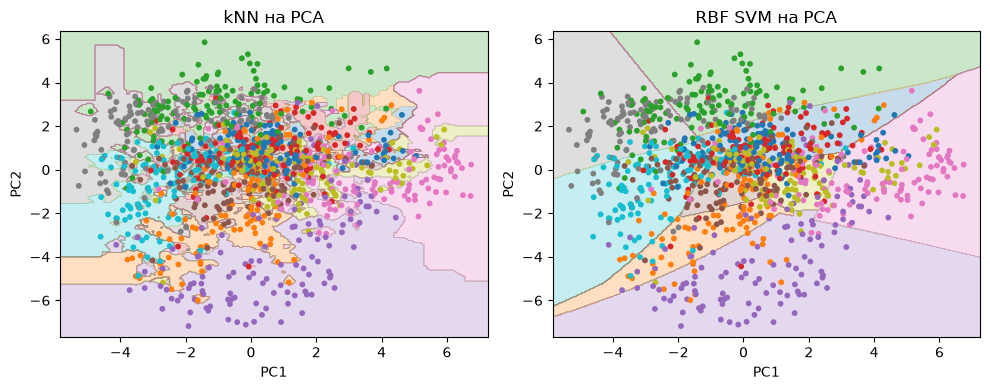
\includegraphics[width=\textwidth]{images/pca_regions.png}
\caption{Решающие области визуализационных моделей kNN и RBF SVM на PCA-проекции (точки --- объекты Train)}
\label{fig:pca}
\end{figure}

Классы в плоскости двух главных компонент сильно перекрываются: на них приходится лишь 17.2\% дисперсии. Области kNN фрагментированы и имеют рваные границы в центре, где классы перемешаны; области RBF SVM заметно более гладкие и ограничены выпуклыми полосами.

\subsection{Финальная оценка на тестовой выборке}

По validation macro-F1 выбран RBF SVM ($C=10$, $\gamma=0.01$): 0.9775 против 0.9628 у kNN и 0.9625 у линейного SVM. Весь Pipeline выбранной модели переобучен на Train+Validation (1600 объектов), Test (400 объектов) использован один раз. Результат: Accuracy = 0.9775, balanced accuracy = 0.9775, macro-F1 = 0.9774. Отчёт по классам --- в таблице~\ref{tab:report}, нормированная confusion matrix --- на рисунке~\ref{fig:cm}.

\begin{table}[h!]
\centering
\begin{tabular}{cccrc}
\toprule
Класс & Precision & Recall & F1-score & Support \\
\midrule
1  & 1.000 & 0.975 & 0.987 & 40 \\
2  & 0.975 & 0.975 & 0.975 & 40 \\
3  & 1.000 & 1.000 & 1.000 & 40 \\
4  & 0.952 & 1.000 & 0.976 & 40 \\
5  & 0.976 & 1.000 & 0.988 & 40 \\
6  & 0.973 & 0.900 & 0.935 & 40 \\
7  & 1.000 & 1.000 & 1.000 & 40 \\
8  & 0.952 & 1.000 & 0.976 & 40 \\
9  & 1.000 & 0.950 & 0.974 & 40 \\
10 & 0.951 & 0.975 & 0.963 & 40 \\
\midrule
Accuracy     &       &       & 0.978 & 400 \\
Macro avg    & 0.978 & 0.977 & 0.977 & 400 \\
Weighted avg & 0.978 & 0.978 & 0.977 & 400 \\
\bottomrule
\end{tabular}
\caption{Отчёт о классификации (RBF SVM, test)}
\label{tab:report}
\end{table}

\begin{figure}[h!]
\centering
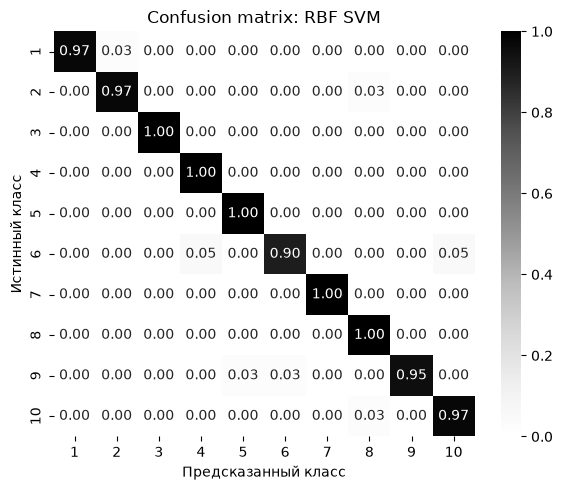
\includegraphics[width=0.62\textwidth]{images/confusion_matrix.png}
\caption{Нормированная матрица ошибок (доля объектов истинного класса) RBF SVM на test}
\label{fig:cm}
\end{figure}

Слабее всего распознаётся класс 6 (recall = 0.900, 4 ошибки из 40: по две в классы 4 и 10); по одной ошибке в классах 1, 2 и 10 и две в классе 9 (в классы 5 и 6). Классы 3, 4, 5, 7 и 8 распознаны полностью.

\subsection{Анализ ошибок}

Из 400 тестовых объектов ошибочно классифицированы 9 (таблица~\ref{tab:errors}); все они разобраны. Столбец Idx --- позиция объекта в тестовой выборке.

\begin{table}[h!]
\centering
\begin{tabular}{rcrrrrr}
\toprule
Idx & true & pred & att1 & att2 & att4 & att7 \\
\midrule
24  & 6  & 10 & $-4.55$ & $-1.73$ & $6.74$  & $-2.47$ \\
66  & 6  & 4  & $11.58$ & $5.12$  & $-0.14$ & $2.17$ \\
90  & 6  & 10 & $8.75$  & $-1.32$ & $-4.53$ & $-6.78$ \\
92  & 10 & 8  & $5.65$  & $-8.69$ & $0.05$  & $1.43$ \\
98  & 6  & 4  & $-0.27$ & $-2.90$ & $13.62$ & $-0.74$ \\
103 & 9  & 6  & $-1.11$ & $-7.36$ & $-5.16$ & $-3.34$ \\
123 & 1  & 2  & $-4.79$ & $3.22$  & $0.62$  & $8.06$ \\
212 & 2  & 8  & $5.30$  & $5.30$  & $0.46$  & $-2.22$ \\
341 & 9  & 5  & $-0.33$ & $0.89$  & $-2.64$ & $-6.44$ \\
\bottomrule
\end{tabular}
\caption{Ошибки RBF SVM на test}
\label{tab:errors}
\end{table}

Возможные причины ошибок (отклонение значения указано в стандартных отклонениях истинного класса от его среднего по всем 2000 объектам):
\begin{enumerate}
\item \textbf{Широкий разброс класса 6.} Четыре из девяти ошибок приходятся на класс 6 (объекты 24, 66, 90, 98), у которого, как видно на рисунке~\ref{fig:features}, широкий разброс по \texttt{att1}. Объект 66 (att1 = 11.58, att2 = 5.12) удалён от центра класса 6 на 2.4 и 2.8 отклонения по \texttt{att1} и \texttt{att2}, объект 90 (att1 = 8.75) --- на 1.9 по \texttt{att1}; у объекта 98 значение att4 = 13.62 отклоняется от среднего класса 6 на 3.5.
\item \textbf{Нетипичные значения отдельных признаков.} Объекты 123, 341, 103 и 212 имеют значение одного из признаков, далёкое от среднего своего класса: att45 (объект 123) на $-5.0$, att20 (объект 341) на $-5.3$, att48 (объект 103) на $-4.3$, att9 (объект 212) на $+4.2$. Близкие отклонения у объектов 24 (att20, $-3.7$) и 92 (att60, $-3.2$).
\item \textbf{Перекрытие классов.} Ошибки приходятся на пары классов 6 и 4, 6 и 10, 10 и 8, которые на рисунке~\ref{fig:pca} перемешаны в центре проекции.
\end{enumerate}

% ---------------- Выводы ----------------
\section*{Выводы}
\addcontentsline{toc}{section}{Выводы}

\begin{enumerate}
\item Константный baseline дал на validation Accuracy = 0.1000, balanced accuracy = 0.1000 и macro-F1 = 0.0182 --- нижнюю границу для всех моделей.
\item Масштаб признаков критичен для расстояний: при умножении att2 на 100 kNN без стандартизации снижает validation macro-F1 до 0.5515, доля общих соседей с эталоном падает до 0.0818; со стандартизацией macro-F1 остаётся 0.9403, соседи совпадают полностью (1.0000).
\item Ручной kNN (NumPy, $k=5$, веса по расстоянию, $p=2$) совпал с \texttt{KNeighborsClassifier} на 50 из 50 объектов Validation (доля совпадений 1.0).
\item Лучшие параметры kNN: $k=3$, weights = distance, $p=1$ (CV macro-F1 = $0.9407\sd 0.0120$, validation macro-F1 = 0.9628); с ростом $k$ качество убывает, при $k=31$ CV macro-F1 = 0.9246 (distance, $p=1$).
\item RBF-ядро превосходит линейное: RBF SVM ($C=10$, $\gamma=0.01$) --- CV macro-F1 = $0.9700\sd 0.0119$, validation macro-F1 = 0.9775, 790 опорных векторов (65.8\% Train); линейный SVM ($C=0.01$) --- 0.9549, 0.9625 и 696 опорных векторов (58.0\%); при $\gamma=1$ CV macro-F1 RBF-SVM не превышает 0.1028.
\item Вычислительная стоимость: fit --- 11.35 мс (kNN), 27.67 мс (linear SVM), 40.50 мс (RBF SVM); predict на 1000 объектов --- 32.33, 22.85 и 59.57 мс соответственно; kNN хранит 1200 объектов, SVM --- 696 и 790 опорных векторов.
\item На test выбранный RBF SVM (Train+Validation, 1600 объектов) показал Accuracy = 0.9775, balanced accuracy = 0.9775, macro-F1 = 0.9774; ошибок 9 из 400, слабее всего распознаётся класс 6 (recall = 0.900, 4 ошибки).
\item Протокол соблюдён: SEED = 42, разбиение 60/20/20 (1200/400/400), preprocessing включён в Pipeline и обучался только на Train (затем на Train+Validation), конфигурация выбрана по validation, test использован один раз. PCA-визуализация (доля дисперсии 17.2\%) построена на отдельных двумерных моделях.
\end{enumerate}

\end{document}
